As depicted in \fig{recommender}, a common first step of building a recommender is to capture user-item events and translate them into matrix representation. Here, \texttt{Recommendation.jl} eases the step by providing a unified wrapper called \texttt{DataAccessor}. Since data for recommender systems is easily standardizable as a collection of a user, item, and auxiliary attributes, the common interface helps developers to follow the separation-of-concerns principle and ensure the easiness and reliability of data manipulation. 

To be more precise, raw data is always converted into a \texttt{DataAccessor} instance at the data preprocessing phase with proper validation (e.g., data type check, missing value handling), and hence the subsequent steps can simply take the instance, and access the data (or metadata) without worrying about unexpected input. \fig{accessor} illustrates the procedure.

\begin{figure}[htbp]
    \centering
    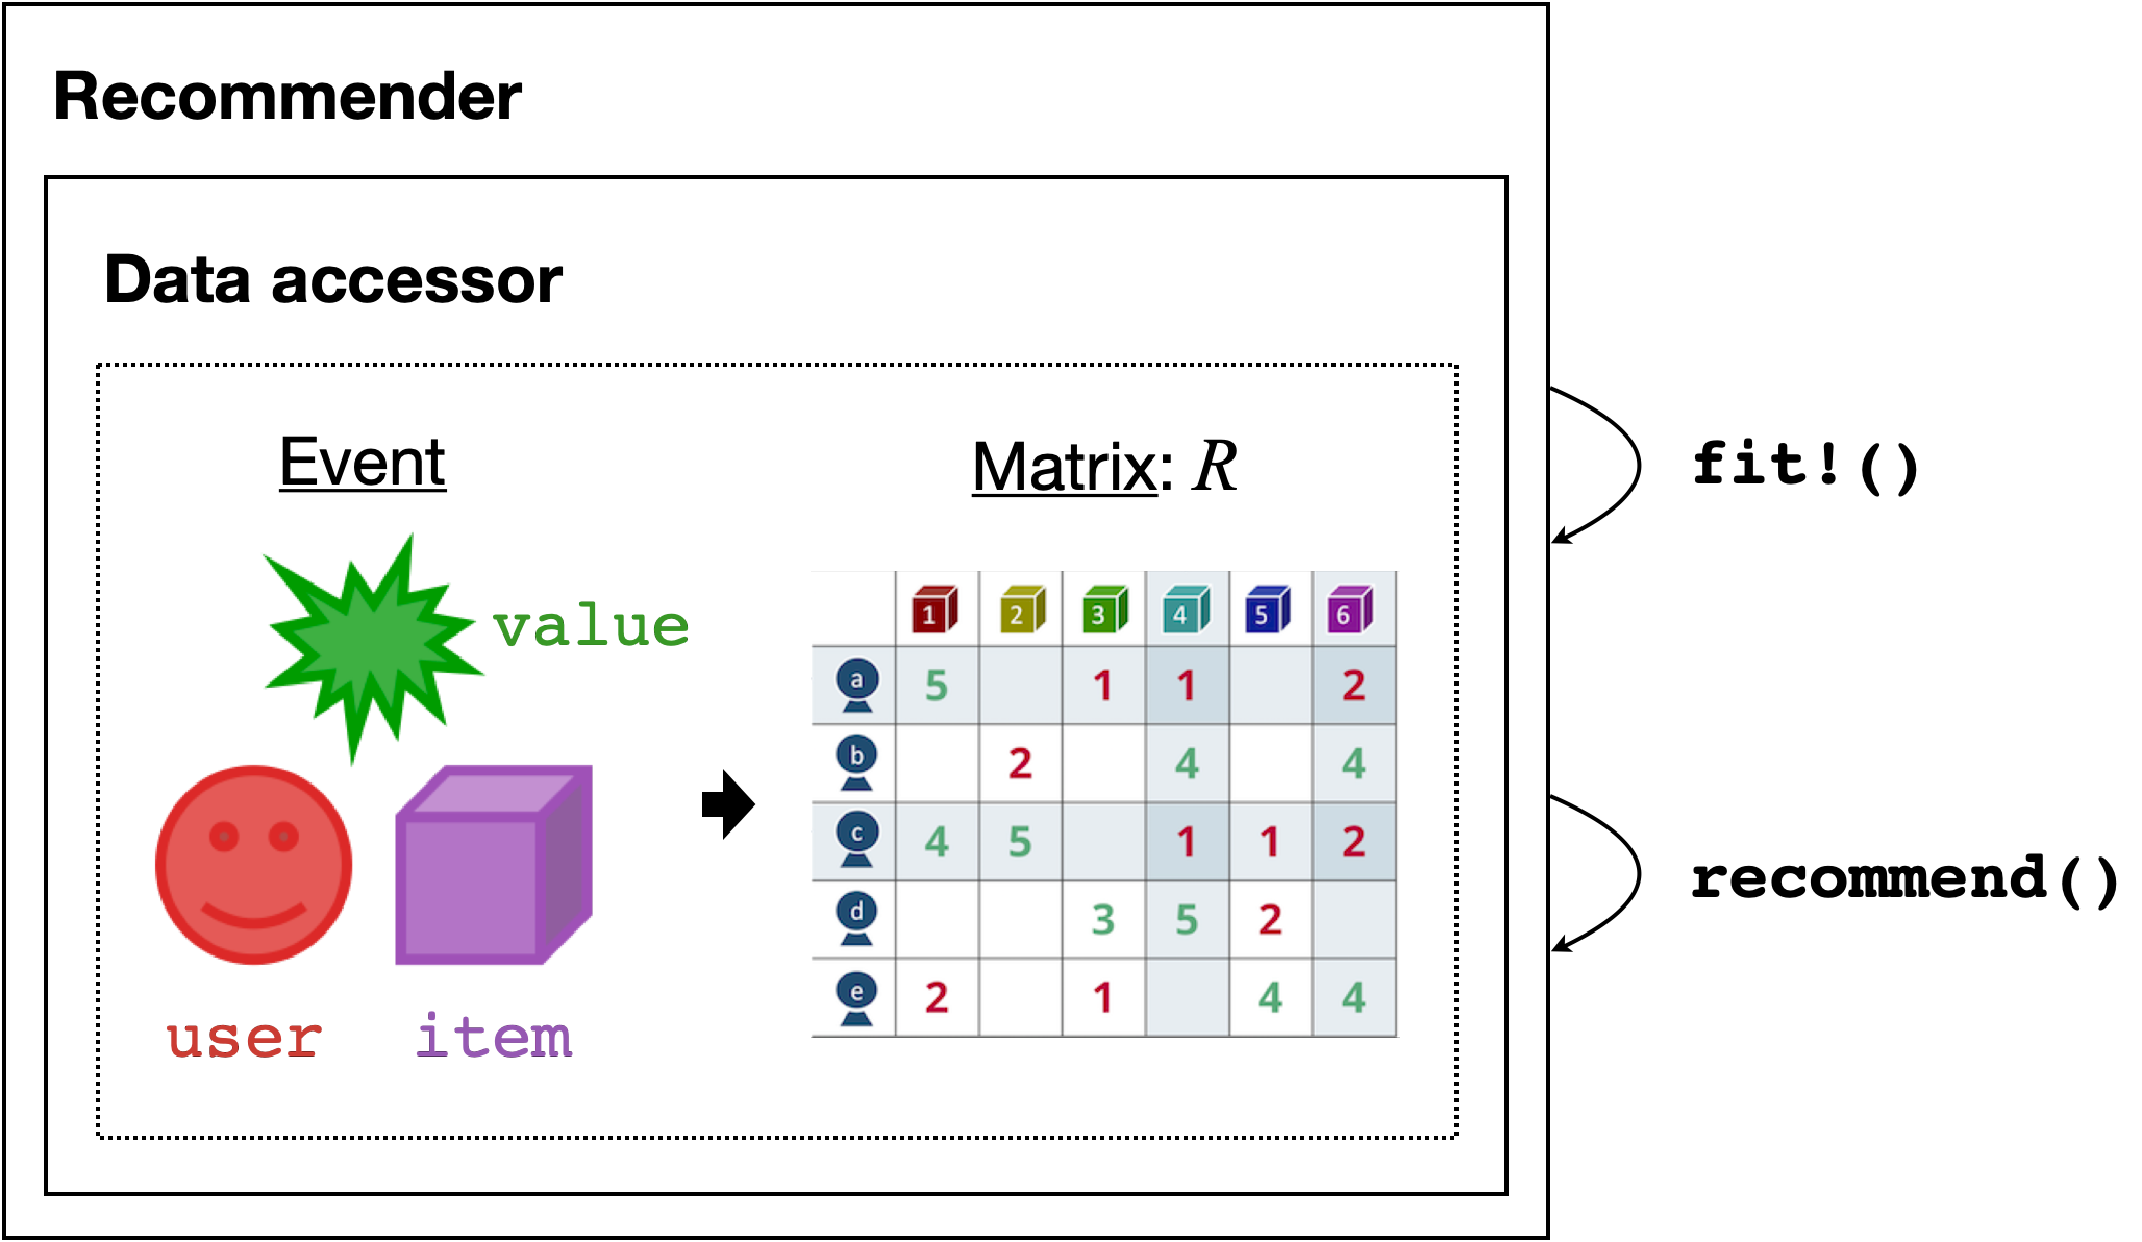
\includegraphics[width=0.8\linewidth]{images/accessor.pdf}
    \caption{\texttt{Recommendation.jl} sees user-item data as a matrix. A recommender runs a training operation \texttt{fit!()} over the data, and a final recommendation list is generated by \texttt{recommend()} based on the trained model.}
    \label{fig:accessor}
\end{figure}

For example, imagine there are 5 users and 6 items on a system, and you observed multiple events:

\begin{lstlisting}[language = Julia]
using Recommendation

n_users, n_items = 5, 6
events = [
    Event(1, 1, 5), # user 1 x item 1
    Event(1, 3, 1), # user 1 x item 3
    # ...
    Event(5, 5, 4), # user 5 x item 5
    Event(5, 6, 4)  # user 5 x item 6
]
\end{lstlisting}

where \texttt{Event} is a composite type for a single user-item interaction:

\begin{lstlisting}[language = Julia]
mutable struct Event
    user::Integer
    item::Integer
    value::Infinite
end
\end{lstlisting}

Note that \texttt{Infinite} is a custom type defined by a union of \texttt{Integer} and \texttt{AbstractFloat}. If \texttt{value} is 0/1 unary integer, such an event is called \textit{implicit feedback,} whereas real numbers like rating value can be seen as the user's \textit{explicit feedback.} Finally, a \texttt{DataAccessor} instance can be created by passing the event list to a constructor as follows, where an array of \texttt{Event} and matrix $R$ are interchangeable.

\begin{lstlisting}[language = Julia]
struct DataAccessor
    events::Array{Event,1}
    R::AbstractMatrix
    user_attributes::Dict{Int,Any}
    item_attributes::Dict{Int,Any}
    
    # constructors
end

data = DataAccessor(events, n_users, n_items)
\end{lstlisting}

In case user (item) data comes with custom attributes such as demographics and contextual metadata, we can use dedicated setter interfaces for enrichment, which allow \texttt{Recommendation.jl} to work with a variety of public and proprietary datasets:

\begin{lstlisting}[language = Julia]
set_user_attribute(data::DataAccessor, 
                   user::Integer, 
                   attribute::AbstractVector)
\end{lstlisting}

Additionally, the package provides data loaders that import publicly available datasets such as MovieLens \cite{harper2015movielens}, Amazon Reviews \cite{ni2019justifying}, and HetRec 2011 Last.FM\footnote{\url{https://www.last.fm/}} dataset \cite{Cantador:RecSys2011}, as well as a synthetic implicit feedback generator using a simple rule-based method demonstrated in \cite{Aharon2013}. These modules return a ready-to-use \texttt{DataAccessor} instance for easing experiments.
